\documentclass[14pt]{beamer}

\usepackage[utf8]{inputenc}

%Information to be included in the title page:
\title{\'Arvores geradoras com poucas ramifica\c{c}\~oes}
\author{Gabriel Dahia}
\institute{Universidade Federal da Bahia}
\date{2019}

\begin{document}

\frame{\titlepage}

\begin{frame}
\frametitle{Defini\c{c}\~oes}
\begin{itemize}
\item<1-> $G = (V, E)$: simples, conexo, n\~ao-direcionado, $n$ v\'ertices, $m$ arestas;
\item<2-> $T \in \mathcal{T}(G)$: \'arvore geradora de $G$;
\item<3-> \emph{Ramifica\c{c}\~ao}: v\'ertice com grau superior a 2;
\item<4-> $b(T)$: n\'umero de ramifica\c{c}\~oes em $T$.
\end{itemize}
\end{frame}

\begin{frame}
\frametitle{Problema MBST}
\begin{block}{\textit{Minumum Branches Spanning Tree} (MBST)}
Dado $G = (V, E)$, queremos $T^*$ tal que
\begin{equation}
T^* = \mathrm{arg\,min}_{T \in \mathcal{T}(G)} b(T)
\end{equation}
\end{block}
\end{frame}

\begin{frame}
\frametitle{Problema MBST}
\begin{figure}
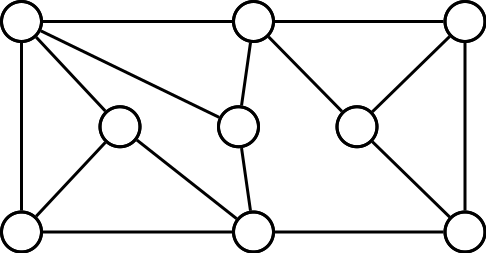
\includegraphics[width=0.7\textwidth]{figures/minbst1.png}
\end{figure}
\end{frame}

\begin{frame}
\frametitle{Problema MBST}
\begin{figure}
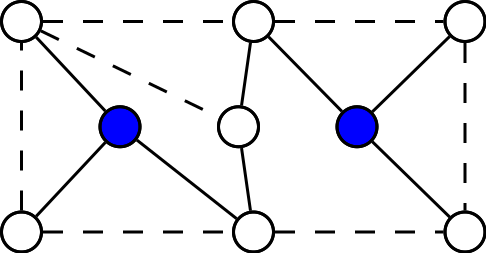
\includegraphics[width=0.7\textwidth]{figures/minbst2.png}
\end{figure}
\end{frame}

\begin{frame}
\frametitle{Problema MBST}
\begin{figure}
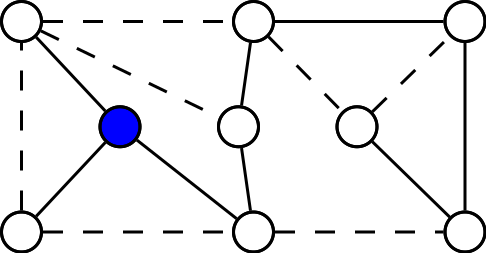
\includegraphics[width=0.7\textwidth]{figures/minbst3.png}
\end{figure}
\end{frame}

\begin{frame}
\frametitle{Problema MBST}
\begin{figure}
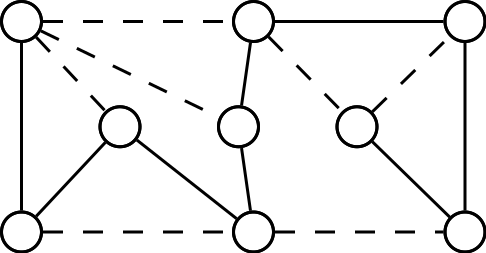
\includegraphics[width=0.7\textwidth]{figures/minbst4.png}
\end{figure}
\end{frame}

\begin{frame}
\frametitle{Aplica\c{c}\~oes}
\begin{itemize}
\item<1-> Vers\~ao do \emph{Caminho Hamiltoniano};
\item<2->Redes \'opticas:
\begin{itemize}
  \item Comunica\c{c}\~ao \textit{multicast};
  \item Multiplexa\c{c}\~ao (DWDM).
\end{itemize}
\end{itemize}
\end{frame}

\begin{frame}
\frametitle{Problemas relacionados}
\begin{itemize}
\item<1->Problema NP-D\'ificil;
\item<2->Caminho Hamiltoniano;
\item<3->Minimizar folhas – maximizar v\'ertices internos;
\item<4->Maximizar v\'ertices n\~ao-ramificantes.
\end{itemize}
\end{frame}

\begin{frame}
\frametitle{T\'ecnicas anteriores}
\begin{itemize}
\item<1->Algoritmos exatos:
\begin{itemize}
\item polinomiais p/ casos espec\'ificos;
\item aproximativos.
\end{itemize}
\item<2->Programa\c{c}\~ao inteira;
\item<3->Heur\'isticas.
\end{itemize}
\end{frame}

\begin{frame}
\frametitle{Heur\'isticas conhecidas}
\begin{itemize}
% ambos sao objetivos validos: se conseguirmos otimizar essas
% quantidades perfeitamente, nos otimizamos MBST. (explicar como)
\item Algoritmos gulosos:
\begin{itemize}
\item arestas que criem menos ramifica\c{c}\~oes;
\item caminhos longos.
\end{itemize}
\end{itemize}
\end{frame}

\end{document}
